\documentclass[letterpaper,12pt]{article}
\usepackage[margin=64pt]{geometry}
\usepackage{amsthm}
\usepackage{amsmath}
\usepackage{amssymb}
\usepackage{parskip}
\usepackage{graphicx}
\usepackage{enumerate}
\usepackage{hyperref}
\usepackage{listings}
\newcommand{\transpose}{^{\mbox{\tiny T}}}


\begin{document}
\thispagestyle{empty}

\hrule \vspace{0.5em}
\noindent {\bf CFRM 462: Introduction to Computational Finance and Econometrics} \hfill Homework 6 \newline \hrule

\vspace{1em}

\begin{enumerate}
\item Efficient Frontiers
\subitem{a)} Boeing and Microsoft \\
	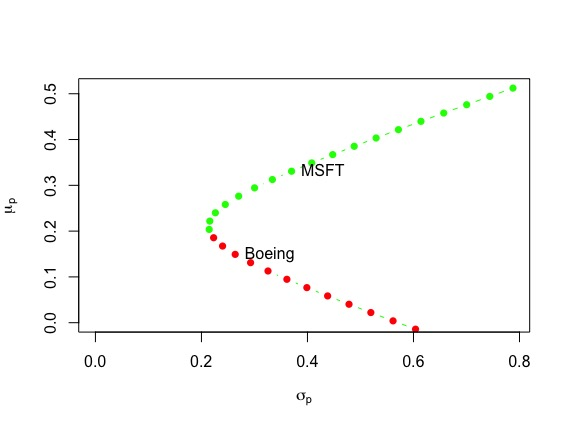
\includegraphics[scale = 0.6]{Boeing_MFST_EF}\\

\subitem{b)} Boeing/MFST and T-Bills Capital Allocation Line \\
	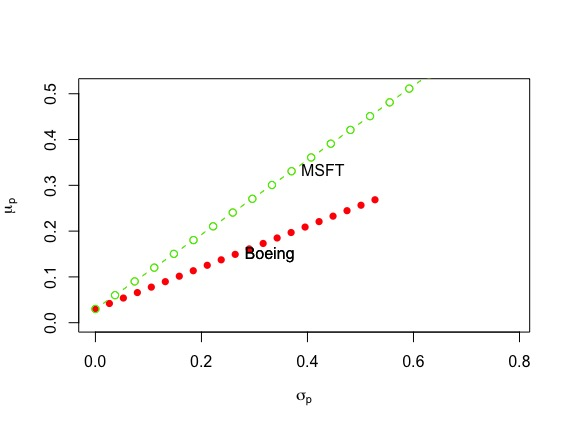
\includegraphics[scale = 0.6]{MFST_BOEING_CAL}

\subitem{c)} The Efficient Frontier\\
	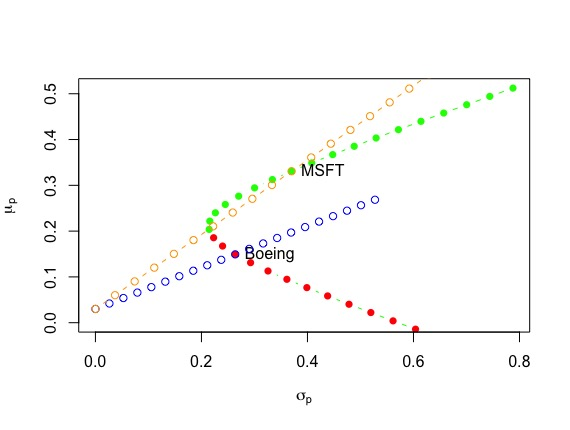
\includegraphics[scale = 0.6]{ALL_EF}

\subitem{d)} The combinations of MFST and T-Bills have expected returns which are uniformly greater than portfolios consisting of T-Bills and Boeing. This occurs because the share ratio for Boeing, $S_B = 0.452145 <$ the sharpe ratio for MFST, $S_M = 0.812778$. 

\item

\end{enumerate}

\vfill \hrule \vspace{2mm} \centerline {\tt \tiny http://computational-finance.uw.edu}
\end{document}